\chapter{Download project from the OpenQuake Platform}

\begin{figure}
    \centering
    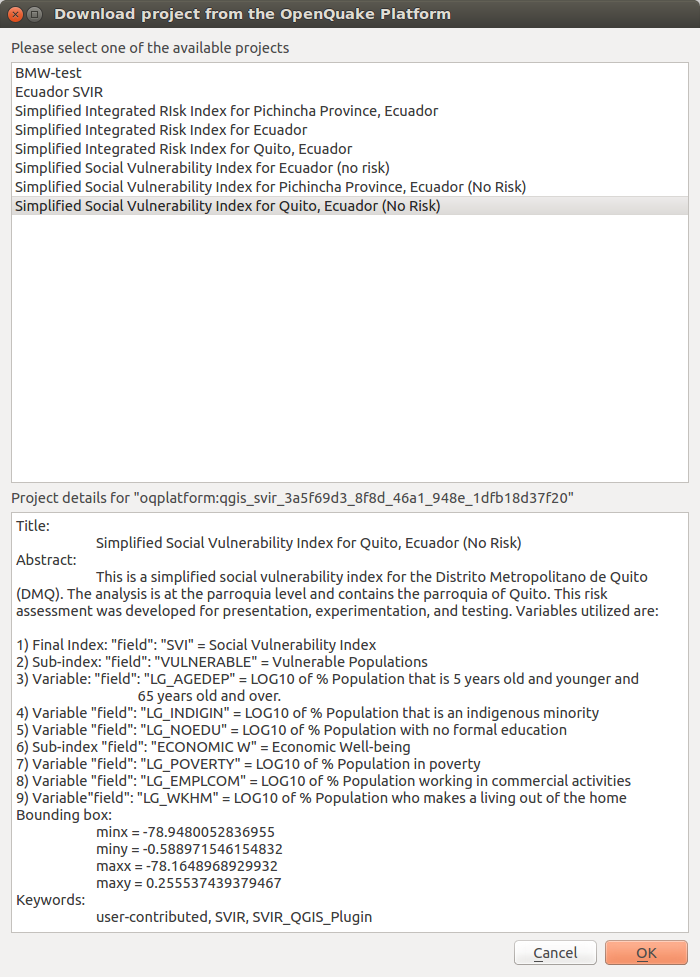
\includegraphics[width=\textwidth]{../images/image15}
    \caption{Download project from the OpenQuake Platform}
    \label{fig:download_project_from_platform}
\end{figure}

An additional option to access data is by downloading projects shared by others
on the OQ-Platform. By clicking the `Download project from the OpenQuake
Platform', the above dialog is opened (Figure 4). Here, a list of available
projects is displayed. The list will contain the titles of projects for which
the user has been granted editing privileges (their own projects or those
shared with them by other users). When a project is selected from the list, its
title, abstract, bounding box and keywords are displayed in the lower textbox
that is utilized to delineate important attributes of the project's definition.
The label directly above the textbox displays an ID that uniquely identifies
the layer used in the OpenQuake-platform.

By pressing `OK', the layer will be downloaded into the QGIS\@. If the associated
project only contains one `project definition', it will be automatically be
selected and downloaded. Otherwise, the project definition manager will open
(see Chapter~\ref{chap:project_definitions_manager}) allowing the user to choose
one of the available project definitions. Once a project definition is
selected, the composite indicators delineated within the project definition are
re-calculated, and the layer is styled and rendered accordingly. This process
may take some time, depending on the complexity of the project.
